\documentclass[11pt,a4paper]{article}

\usepackage[utf8]{inputenc}
\usepackage[T1]{fontenc}
\usepackage[margin=2.5cm]{geometry}
\usepackage{graphicx}
\usepackage{booktabs}
\usepackage{hyperref}

% Print underscores literally in text/\texttt without escaping.
\usepackage[strings]{underscore}

\title{Remote work, team velocity, and long-term capability\\
       \large An agent-based simulation of a 10-developer team}
\author{}
\date{}

\begin{document}
\maketitle

The report is in two parts. Part~A is the original single-sprint model, in which each
developer's skill is fixed; it measures the direct effect of remote work on one sprint's
velocity. Part~B extends the model to a one-year horizon and adds two new mechanisms, learning
and turnover, so that the amount of remote work can affect the team's capability over time and
not only its output in a single sprint.

\section*{Part A: a single sprint}

The simulation is built on Mesa 3.x. One sprint lasts 10 working days, modelled as 320 ticks of
15 minutes each. The team has 10 developers working through a backlog of 500 tasks, with story
points drawn from $\{1,2,3,5\}$ and four ticks of work per point. When a developer hits a blocker
they first try to clear it alone; if that fails they look for a colleague to help. Help between
two people in the office is quick, while help involving someone working from home is slower,
because it happens asynchronously.

Three experiment series were run, each with 20 replications (different random seeds) per cell:

\begin{center}
\begin{tabular}{clccc}
\toprule
\# & Factor(s) & Levels & Replications & Total runs \\
\midrule
1 & \texttt{remote_share} (baseline)            & 11 (0.0--1.0, step 0.1)        & 20 & 220 \\
2 & \texttt{remote_share} $\times$ \texttt{mean_solo_skill} & $6\times3$ (skill $\in\{0.3,0.5,0.7\}$) & 20 & 360 \\
3 & \texttt{remote_share} $\times$ \texttt{block_prob}      & $6\times3$ (bp $\in\{0.01,0.02,0.05\}$)  & 20 & 360 \\
\bottomrule
\end{tabular}
\end{center}

This gives 940 simulations in total. The remaining parameters keep their defaults: office help
takes $1\pm1$ ticks, remote help $5\pm2$ ticks, and individual solo skill is spread by $\pm0.2$
around its mean.

\subsection*{Experiment 1: baseline sweep of \texttt{remote_share}}

As the share of remote work rises from none to everyone, velocity falls steadily and the average
wait for help grows, because more of the help that does happen is the slower, asynchronous kind.

\begin{figure}[htbp]
  \centering
  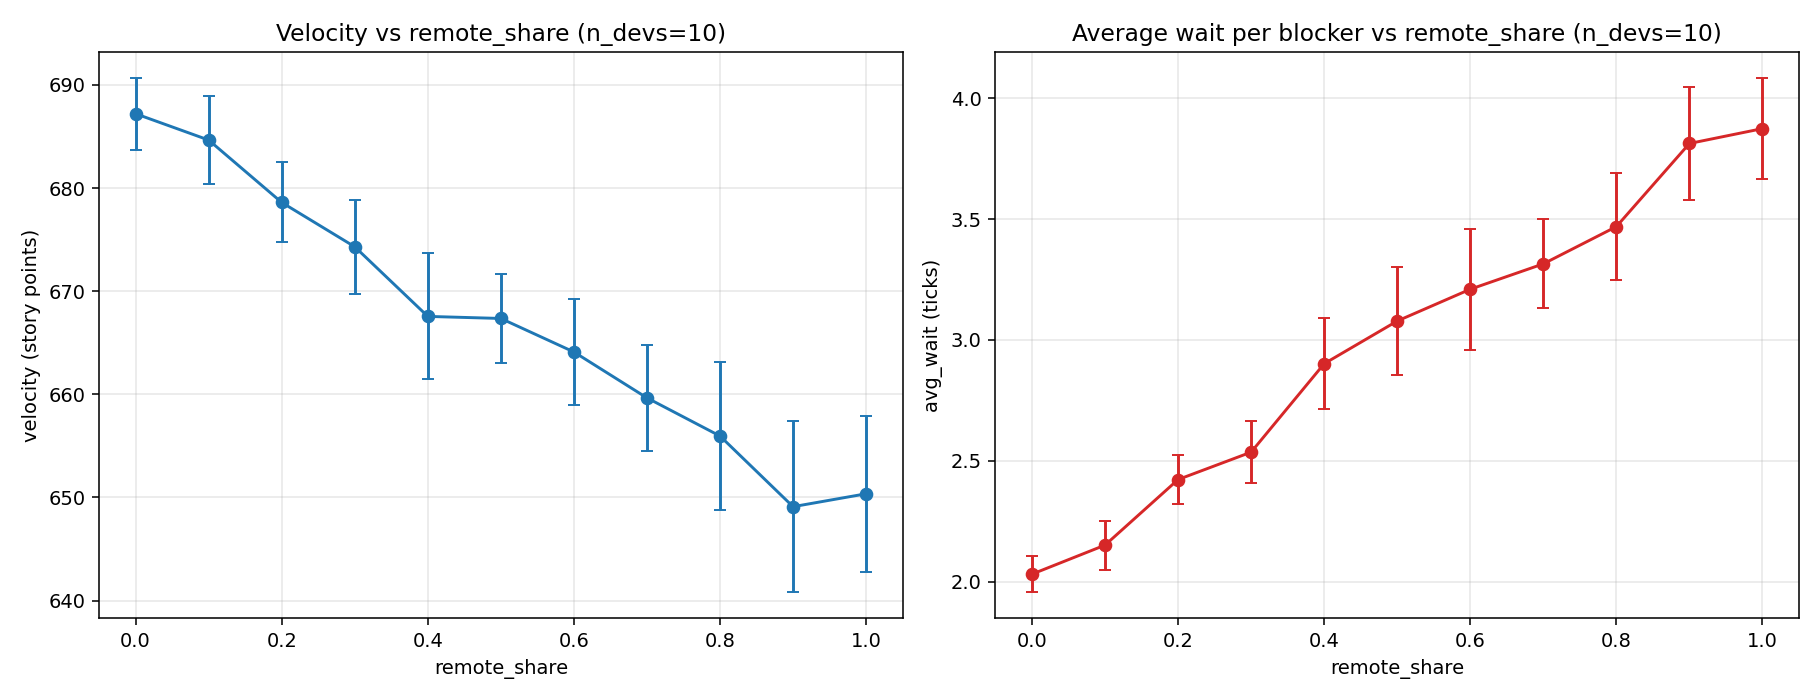
\includegraphics[width=0.82\textwidth]{exp1_baseline.png}
  \caption{Velocity and average wait per blocker against the share of remote work.}
\end{figure}

\begin{center}
\begin{tabular}{cccc}
\toprule
\texttt{remote_share} & velocity (mean $\pm$ CI95) & avg.\ wait & blockers resolved \\
\midrule
0.0 & $687.2 \pm 3.5$ & 2.0 & 52.0 \\
0.3 & $674.3 \pm 4.6$ & 2.5 & 52.3 \\
0.5 & $667.4 \pm 4.3$ & 3.1 & 49.2 \\
0.7 & $659.6 \pm 5.2$ & 3.3 & 50.6 \\
1.0 & $650.4 \pm 7.6$ & 3.9 & 47.5 \\
\bottomrule
\end{tabular}
\end{center}

\subsection*{Experiment 2: remote share and individual skill}

The size of the remote penalty depends on how often people actually need help. A more skilled team
clears most blockers alone and barely notices slower remote help; a less skilled team leans on the
help channel and suffers far more. The velocity lost when moving from a fully office to a fully
remote team ranges from 9.0\% for a low-skill team down to 3.6\% for a high-skill one.

\begin{figure}[htbp]
  \centering
  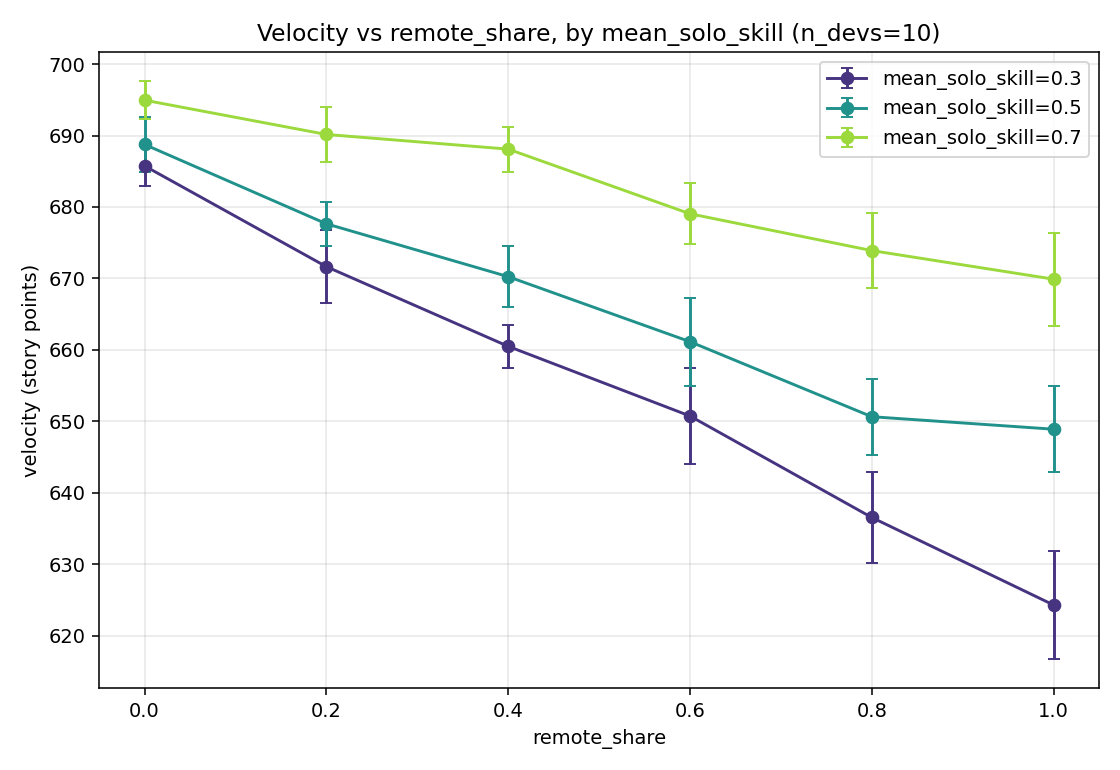
\includegraphics[width=0.62\textwidth]{exp2_skill_interaction.png}
  \caption{Velocity against remote share, grouped by mean solo skill.}
\end{figure}

\begin{center}
\begin{tabular}{ccccc}
\toprule
\texttt{mean_solo_skill} & velocity @ 0\,\% & velocity @ 100\,\% & absolute loss & relative loss \\
\midrule
0.30 & 685.8 & 624.3 & $-61.5$ SP & $-9.0\%$ \\
0.50 & 688.8 & 648.9 & $-39.9$ SP & $-5.8\%$ \\
0.70 & 695.0 & 669.9 & $-25.1$ SP & $-3.6\%$ \\
\bottomrule
\end{tabular}
\end{center}

\subsection*{Experiment 3: remote share and blocker frequency}

For the same reason, the penalty grows sharply with how often blockers occur. When blockers are
rare the help channel is used little and remote work costs about 3\%; when they are frequent the
team is constantly waiting for help and the cost rises to roughly 13\%.

\begin{figure}[htbp]
  \centering
  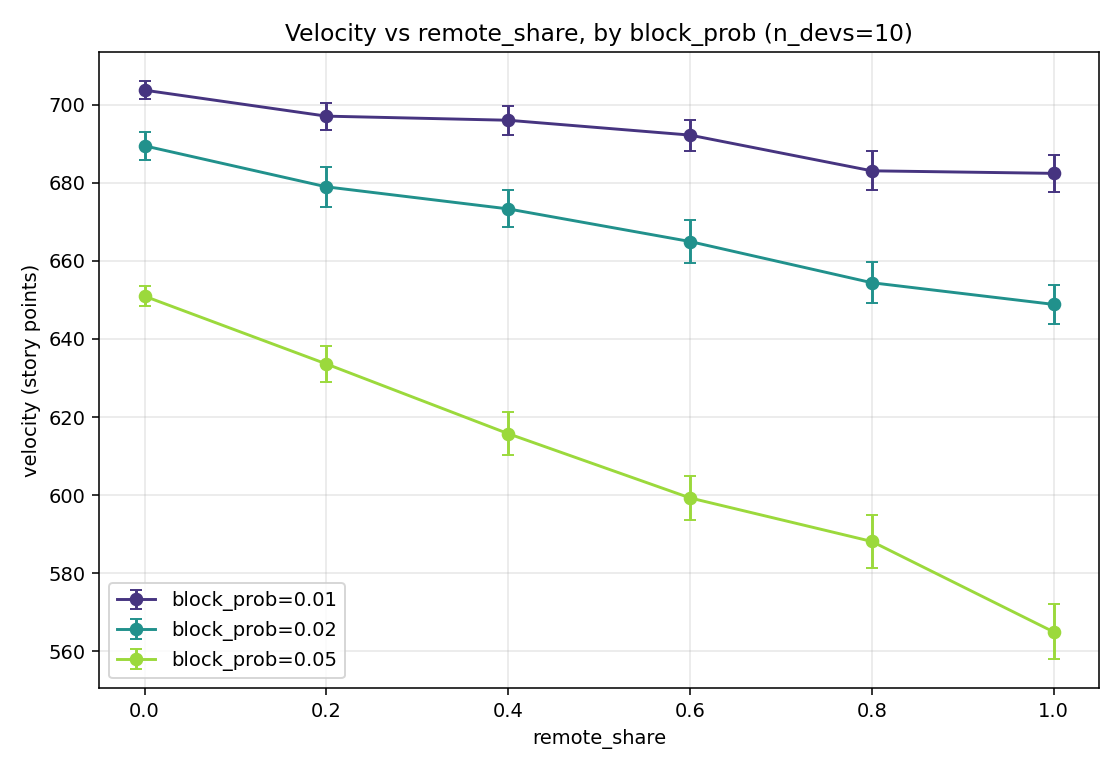
\includegraphics[width=0.62\textwidth]{exp3_blockprob_interaction.png}
  \caption{Velocity against remote share, grouped by blocker probability.}
\end{figure}

\begin{center}
\begin{tabular}{ccccc}
\toprule
\texttt{block_prob} & velocity @ 0\,\% & velocity @ 100\,\% & absolute loss & relative loss \\
\midrule
0.01 & 703.7 & 682.4 & $-21.3$ SP & $-3.0\%$ \\
0.02 & 689.5 & 648.9 & $-40.6$ SP & $-5.9\%$ \\
0.05 & 651.0 & 565.0 & $-86.0$ SP & $-13.2\%$ \\
\bottomrule
\end{tabular}
\end{center}

\section*{Part B: a year, with learning and turnover}

Part~A treats each developer's skill as fixed. Over a single sprint that is fine, but over a year
it is not, because people get better at their work and teams lose and gain members. Part~B adds
two mechanisms so that the model can run over a longer horizon (24 two-week sprints, about a year)
and so that the amount of remote work can shape the team's capability, not just its immediate
output.

\subsection*{How the two mechanisms work}

\paragraph{Learning.} Each developer has a skill level, which is simply the chance that they can
clear a blocker on their own without asking anyone. In Part~A this number never changes; here it
grows with experience. Every time a developer finishes a task or resolves a blocker, their skill
takes a small step towards a ceiling, and the steps get smaller as they approach it. The result is
fast progress at first and then a plateau, matching the pattern in onboarding studies where a new
hire reaches most of their productivity within about six months. The way a blocker is resolved
also matters: help received face to face in the office teaches more than the same help exchanged
asynchronously with someone at home. This is the only route through which remote work slows
learning, so the model needs no separate ``remote learning'' setting.

\paragraph{Turnover.} At the end of each sprint, every developer may leave with a small
probability taken from an annual attrition rate, about 12\% per year in the base case. Anyone who
leaves is replaced straight away by a junior who starts with low skill and has to learn from
scratch, so each departure pulls the team's average skill down and resets part of the learning
curve. The amount of remote work can either raise or lower the chance of leaving. Since the
evidence points both ways, remote work improves retention in one large study and harms it in
another, this is left as an adjustable coefficient and the results are shown for both readings.

\subsection*{What the year-long runs show}

The measure that matters here is cumulative velocity, the total story points delivered over the
whole year rather than in any single sprint. Four sweeps of the remote share were run, again with
20 replications per cell.

Across the year a fully co-located team delivers roughly 2.5\% to 2.8\% more than a fully remote
one. The gap grows steadily with the remote share, but its most telling feature is when it occurs:
it is largest early in the year and shrinks as the team matures.

\begin{center}
\begin{tabular}{lc}
\toprule
Horizon & Advantage of the office team \\
\midrule
6 sprints (about 3 months)  & $+4.7\%$ \\
12 sprints (about 6 months) & $+3.3\%$ \\
24 sprints (about 1 year)   & $+2.6\%$ \\
\bottomrule
\end{tabular}
\end{center}

The reason is that the remote penalty is at heart a penalty on the help channel: remote developers
wait longer for asynchronous help. Learning works against this penalty rather than with it. As
both teams grow more skilled they need help less often, so the channel where remote work loses
ground matters less and less. With learning switched off, the office team's advantage over a year
is 6.2\%; with learning on it falls to 2.5\%. In other words the cost of remote work is
concentrated in the early, junior, frequently-blocked phase and fades once the team is
experienced. This is the reverse of the compounding effect that seemed likely before the model was
run.

\begin{figure}[htbp]
  \centering
  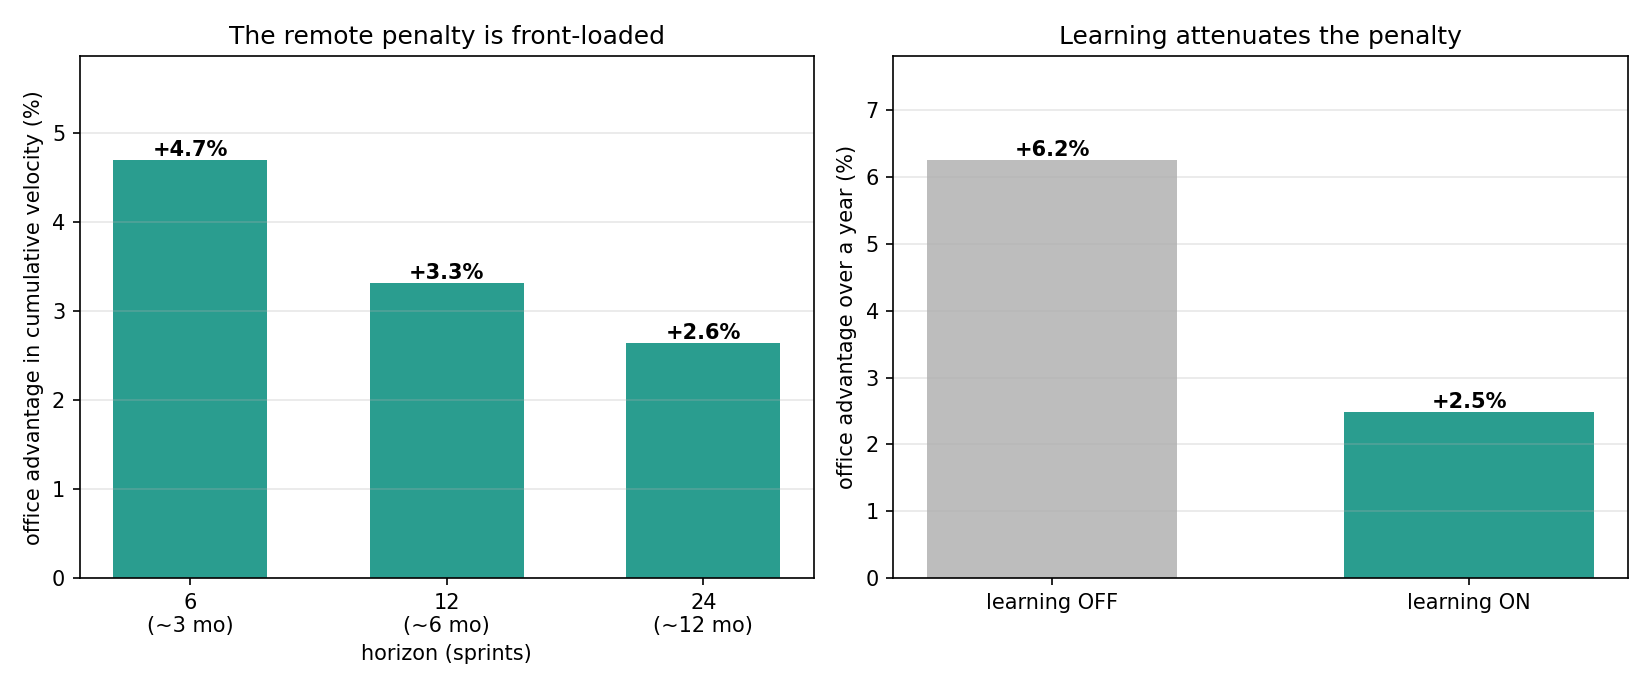
\includegraphics[width=0.88\textwidth]{partb_penalty.png}
  \caption{The office advantage in cumulative velocity is largest early and shrinks over the year
  (left); switching learning on more than halves it (right).}
\end{figure}

\begin{figure}[htbp]
  \centering
  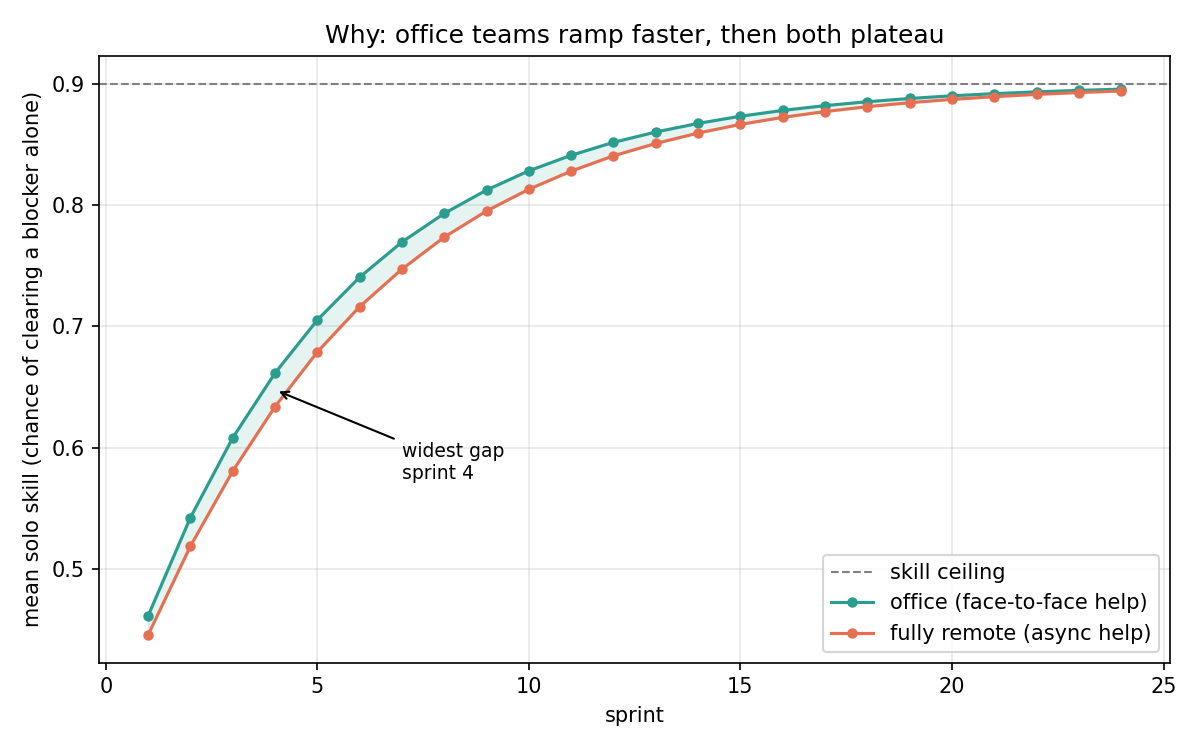
\includegraphics[width=0.6\textwidth]{partb_skillramp.png}
  \caption{Mean solo skill over the year for a team of juniors. The office team ramps a little
  faster, but both reach the same ceiling, so the gap is widest mid-ramp and closes by year end.}
\end{figure}

The turnover coefficient behaves as designed. Under the retention reading, where remote work helps
keep people, a fully remote team loses fewer members over the year than an office team; under the
isolation reading, where remote work pushes juniors out, it loses more.

\begin{center}
\begin{tabular}{ll}
\toprule
Scenario & departures: office $\to$ fully remote \\
\midrule
retention (remote keeps people)   & $1.9 \to 0.7$ \\
isolation (remote pushes them out) & $0.6 \to 2.0$ \\
\bottomrule
\end{tabular}
\end{center}

\begin{figure}[htbp]
  \centering
  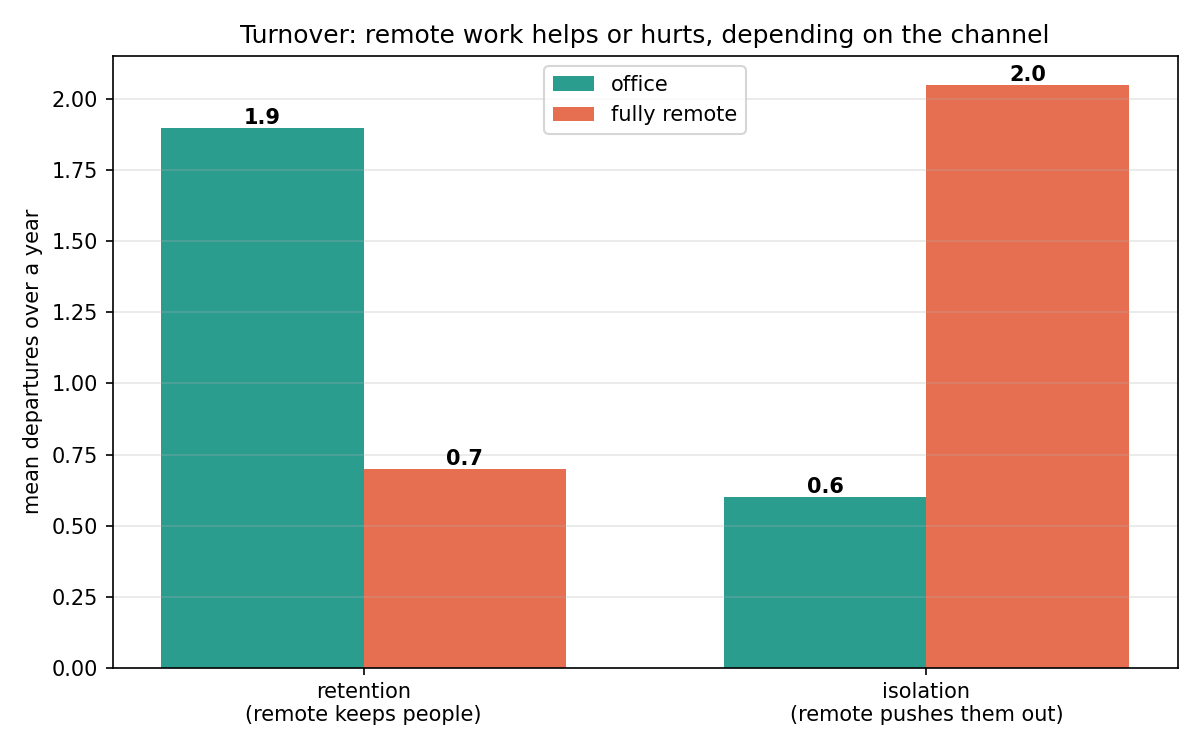
\includegraphics[width=0.6\textwidth]{partb_turnover.png}
  \caption{Departures over a year, office versus fully remote, under the two readings of how remote
  work affects retention.}
\end{figure}

Taken together, the model does not claim that remote work is simply good or bad for output. Its
cost depends on the state of the team: it is small for an experienced and stable team, and largest
for a junior-heavy team with high turnover that is still climbing the learning curve.

\section*{The interactive interface}

The model ships with two interactive front-ends, both driven by the same simulation code. The
original one (\texttt{app.py}, run with \texttt{solara run app.py}) exposes every parameter as a
slider and plots the five time series discussed below. A second, richer front-end
(\texttt{app_streamlit.py}, run with \texttt{streamlit run app_streamlit.py}) keeps those same
sliders and charts but adds an animated view of the team, so that the mechanisms behind the
aggregate curves can be watched directly. This section documents the whole interface: every
parameter, every chart, and the animation.

The layout is the same in both: parameters live in a sidebar, grouped into collapsible sections,
and the charts (and, in the Streamlit version, the animation) fill the main area. Changing any
parameter re-runs the simulation and redraws everything.

\subsection*{Parameters}

The sidebar groups the parameters by role. The headline variable is \texttt{remote_share}; the
remaining groups set up the team, the work process, learning, turnover, and the run itself. Each
slider's default and range are given alongside what it controls.

\begin{center}
\begin{tabular}{llp{8.0cm}}
\toprule
Parameter & Default (range) & What it controls \\
\midrule
\multicolumn{3}{l}{\textit{Headline}}\\
\texttt{remote_share} & 0.5 (0--1) & Probability each developer works from home on a given day, rolled afresh every morning. The policy variable under study. \\
\addlinespace
\multicolumn{3}{l}{\textit{Team heterogeneity}}\\
\texttt{mean_solo_skill} & 0.5 (0--1) & Team-mean solo skill: the chance a developer clears a blocker alone, without asking for help. \\
\texttt{solo_skill_spread} & 0.2 (0--0.5) & Half-width of the uniform spread of solo skill across developers, around the mean. \\
\addlinespace
\multicolumn{3}{l}{\textit{Process}}\\
\texttt{block_prob} & 0.02 (0--0.10) & Per-tick probability that a working developer hits a blocker. \\
\texttt{sync_help_mean} & 1 (0--5) & Mean length, in ticks, of a co-located (office-to-office) help session. \\
\texttt{async_help_mean} & 5 (1--20) & Mean length, in ticks, of a help session involving anyone working from home. \\
\addlinespace
\multicolumn{3}{l}{\textit{Learning}}\\
\texttt{learning_rate} & 0.0123 (0--0.05) & Size of the skill step taken on each learning event; calibrated so a junior closes about 90\% of the gap to the ceiling in roughly 12 sprints. Set to 0 to switch learning off. \\
\texttt{skill_cap} & 0.90 (0.5--1.0) & Ceiling that solo skill approaches but never exceeds. \\
\texttt{sync_help_weight} & 1.5 (0--3) & Multiplier on the skill gained when a blocker is resolved through co-located help. \\
\texttt{async_help_weight} & 1.0 (0--3) & Same multiplier for remote help; lower than the sync weight, so remote help teaches less. \\
\addlinespace
\multicolumn{3}{l}{\textit{Turnover}}\\
\texttt{annual_attrition} & 0.12 (0--0.30) & Annual probability that a developer leaves, converted internally to a per-sprint hazard. \\
\texttt{junior_mean_skill} & 0.40 (0--0.8) & Skill of a newly hired replacement, as a fraction of the skill ceiling. \\
\texttt{remote_attrition_coef} & 0.0 ($-1$--1) & Sign and size of remote work's effect on leaving: positive raises attrition with remote share (isolation reading), negative lowers it (retention reading). \\
\addlinespace
\multicolumn{3}{l}{\textit{Structural}}\\
\texttt{n_devs} & 5 (2--10) & Number of developers on the team. \\
\texttt{sprint_length} & 320 (32--640) & Ticks per sprint; 320 is ten working days at 32 ticks (15 minutes each) per day. \\
\texttt{n_sprints} & 24 (1--52) & Number of sprints in the run; 24 two-week sprints is about a year. \\
\texttt{sp_scaling_k} & 4 (1--16) & Ticks of work per story point. \\
\addlinespace
\multicolumn{3}{l}{\textit{Reproducibility}}\\
\texttt{seed} & 42 (0--10000) & Random-number seed; fixing it makes a run exactly repeatable. \\
\bottomrule
\end{tabular}
\end{center}

\subsection*{Charts}

The five charts are time series over ticks, read straight from the model's data collector. They are
the same in both front-ends.

\begin{center}
\begin{tabular}{p{4.6cm}p{10.4cm}}
\toprule
Chart & What it shows \\
\midrule
Per-sprint velocity & Story points completed inside the current sprint, resetting to zero at each sprint boundary; the saw-tooth height is that sprint's throughput. \\
Mean waiting time per resolved blocker & Running mean of the ticks elapsed between hitting a blocker and clearing it. It rises with the share of remote work, because more help arrives through the slower asynchronous channel. \\
Developer states over time & Number of developers in each state each tick---working, blocked, helping, idle---using the same colours as the node fills in the animation. \\
Team skill over time & Mean, minimum, and maximum solo skill across the team. The upward ramp is learning; the downward steps are turnover, as an experienced leaver is replaced by a low-skill junior. \\
Attrition and tenure & Cumulative number of departures and the team's mean tenure (ticks since each current member was hired). \\
\bottomrule
\end{tabular}
\end{center}

\subsection*{The animated team view (Streamlit only)}

Each developer is drawn as a node spaced evenly around a circle. A node carries two independent
colour channels. Its \emph{inner fill} encodes what the developer is doing this tick---idle,
working, blocked, or helping someone else---using the same colours as the ``developer states''
chart. Its \emph{outer ring} encodes where the developer is working today, in the office or from
home; this is the single distinction that decides whether a help session is fast and co-located or
slow and asynchronous, so it is given its own visual channel rather than being folded into the
fill.

When one developer is blocked and another steps in to help, an \emph{edge} is drawn between the two
nodes for as long as the help session lasts. The edge is solid when both people are in the office
(a synchronous session) and dashed when at least one is remote (an asynchronous one). At a glance
the picture therefore shows how much of the team is productive versus waiting, how the office/home
split falls on any given day, and how much of the help that is happening is the slower remote kind:
the very quantities whose averages drive the velocity and waiting-time curves above.

\begin{figure}[htbp]
  \centering
  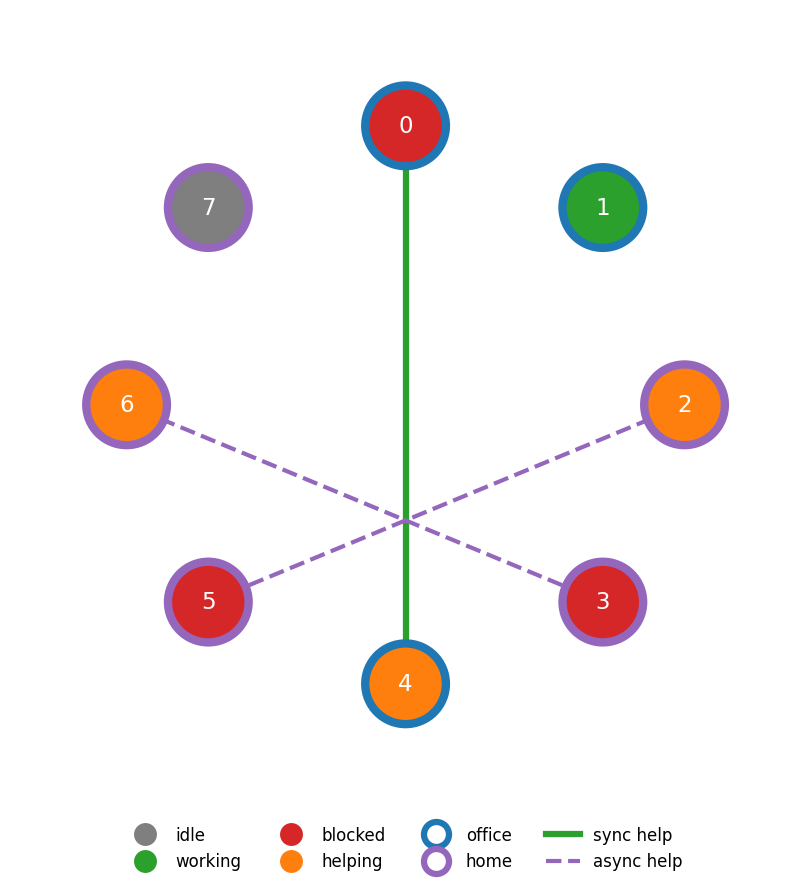
\includegraphics[width=0.66\textwidth]{interface_screenshot.png}
  \caption{A single tick of the animated team view. Inner fill is the developer's state and the
  outer ring is their location; a solid edge is a co-located (sync) help session and a dashed edge a
  remote (async) one. Here developer~0 is being helped in the office while developers~3 and~5,
  working from home, wait on slower asynchronous help.}
\end{figure}

Streamlit does not animate while a model is stepping, so the run and the playback are separated. On
any change of parameters the model is executed once to completion and the state of every developer
is recorded at each tick; the recording is then replayed through the play/pause controls and the
time slider below the figure, with no recomputation while scrubbing. The number of recorded frames
is sub-sampled (a sidebar slider sets the cap) so that long horizons stay responsive in the
browser, and the result is cached on the parameter set, so moving the slider or pressing play never
re-runs the simulation.

\end{document}
